%% Exemplo de utilizacao do estilo de formatacao normas-utf-tex (http://normas-utf-tex.sourceforge.net)
%% Autores: Hugo Vieira Neto (hvieir@utfpr.edu.br)
%%          Diogo Rosa Kuiaski (diogo.kuiaski@gmail.com)
%% Colaboradores:
%%          Cézar M. Vargas Benitez <cesarvargasb@gmail.com>
%%          Marcos Talau <talau@users.sourceforge.net>


\documentclass[openright]{normas-utf-tex} %openright = o capitulo comeca sempre em paginas impares
%\documentclass[oneside]{normas-utf-tex} %oneside = para dissertacoes com numero de paginas menor que 100 (apenas frente da folha) 


\usepackage[alf,abnt-emphasize=bf,bibjustif,recuo=0cm, abnt-etal-cite=2, abnt-etal-list=99]{abntcite} %configuracao correta das referencias bibliograficas.

\usepackage[brazil]{babel} % pacote portugues brasileiro
\usepackage[utf8]{inputenc} % pacote para acentuacao direta
\usepackage{amsmath,amsfonts,amssymb} % pacote matematico
\usepackage{graphicx} % pacote grafico
%\usepackage{times} % fonte times

%Podem utilizar GEOMETRY{...} para realizar pequenos ajustes das margens. Onde, left=esquerda, right=direita, top=superior, bottom=inferior. P.ex.:
%\geometry{left=3.0cm,right=1.5cm,top=4cm,bottom=1cm} 

% ---------- Preambulo ----------
\instituicao{Universidade Tecnol\'ogica Federal do Paran\'a} % nome da instituicao
\programa{Engenharia de Computação} % nome do programa
\area{Segurança e Redes} % [Engenharia Biom\'edica] ou [Inform\'atica Industrial] ou [Telem\'atica]

\documento{Trabalho de Conclusão de Curso 1} % [Disserta\c{c}\~ao] ou [Tese]
\nivel{Bacharelado} % [Mestrado] ou [Doutorado]
\titulacao{Bacharelado} % [Mestre] ou [Doutor]

\titulo{\MakeUppercase{DETECÇÃO DE ANOMALIAS EM REDES DE COMPUTADORES}} % titulo do trabalho em portugues
\title{\MakeUppercase{COMPUTER NETWORK ANOMALY DETECTION}} % titulo do trabalho em ingles

\autor{BRUNO ANKEN MOROMIZATO ZANINELLO} % autor do trabalho
\cita{ZANINELLO, Bruno Anken Moromizato} % sobrenome (maiusculas), nome do autor do trabalho

\palavraschave{Detecção de anomalias, Redes de computadores, Segurança.} % palavras-chave do trabalho
\keywords{Anomaly detection, Computer network, Security.} % palavras-chave do trabalho em ingles

\comentario{Trabalho de Conclusão de Curso de graduação do curso de Engenharia de Computação da \ABNTinstituicaodata\ - UTFPR, como requisito parcial para a obten\c{c}\~ao do título de bacharel.}



\orientador{Prof. Dr. Lucas Dias Hiera Sampaio} % nome do orientador do trabalho
%\orientador[Orientadora:]{Nome da Orientadora} % <- no caso de orientadora, usar esta sintaxe
%\coorientador{Nome do Co-orientador} % nome do co-orientador do trabalho, caso exista
%\coorientador[Co-orientadora:]{Nome da Co-orientadora} % <- no caso de co-orientadora, usar esta sintaxe
%\coorientador[Co-orientadores:]{Nome do Co-orientador} % no caso de 2 co-orientadores, usar esta sintaxe
%\coorientadorb{Nome do Co-orientador 2}	% este comando inclui o nome do 2o co-orientador

\local{Cornélio Procópio} % cidade
\data{\the\year} % ano automatico


%---------- Inicio do Documento ----------
\begin{document}

\capa % geracao automatica da capa
\folhaderosto % geracao automatica da folha de rosto
%\termodeaprovacao % <- ainda a ser implementado corretamente

% dedicatória (opcional)
\begin{dedicatoria}
Dedico este texto à minha família, que sempre me apoiou de diversas formas em toda a minha trajetória vida.
\end{dedicatoria}

% agradecimentos (opcional)
\begin{agradecimentos}
Agradeço aos meus amigos, sem os quais minha caminhada até este momento certamente teria sido mais árdua, ao meu professor orientador, que me ajudou, apoiou e orientou de maneira impecável neste trabalho e, principalmente, à minha família, sem a qual teria sido impossível chegar a este momento.
\end{agradecimentos}

% epigrafe (opcional)
%\begin{epigrafe}
%"Navegar é preciso; viver não é preciso."

%Fernando Pessoa
%\end{epigrafe}

%resumo
\begin{resumo}
A segurança em redes de computadores é uma área que movimenta grande quantidade de capital no mercado, desde gastos com reparos de danos causados por ataques efetuados a investimentos em proteções para que os ataques não venham a se concretizar. Os estudos acerca de sistemas de detecção de anomalias iniciaram-se em meados da década de 1980 e foram avançando juntamente às novas tendências tecnológicas na área. Atualmente existem sistemas de detecção de anomalias com arquiteturas distribuídas e atuando na nuvem, por exemplo. A proposta deste trabalho é a criação de um sistema de detecção de anomalias em redes de computadores a partir de uma plataforma ou método de aprendizado de máquina que utilizará um baseline como referência para sua atuação.
\end{resumo}

%abstract
\begin{abstract}
Computer network security is an area that involves a great amount of money, from damage repairing costs of effective attacks to investments on protection against attacks to come. Studies about anomaly detection systems began in the mid 1980s and advanced alongside the new technological trends in the area. There are, nowadays, anomaly detection systems with distributed architecture and cloud acting ones, for example. The purpose of this work is the creation of a computer network anomaly detection system utilizing a machine learning platform or method that uses a baseline as its reference.
\end{abstract}

% listas (opcionais, mas recomenda-se a partir de 5 elementos)
%\listadefiguras % geracao automatica da lista de figuras
%\listadetabelas % geracao automatica da lista de tabelas
%\listadesiglas % geracao automatica da lista de siglas
%\listadesimbolos % geracao automatica da lista de simbolos

% sumario
\sumario % geracao automatica do sumario


%---------- Inicio do Texto ----------
% recomenda-se a escrita de cada capitulo em um arquivo texto separado (exemplo: intro.tex, fund.tex, exper.tex, concl.tex, etc.) e a posterior inclusao dos mesmos no mestre do documento utilizando o comando \input{}, da seguinte forma:
%\input{intro.tex}
%\input{fund.tex}
%\input{exper.tex}
%\input{concl.tex}


%---------- Primeiro Capitulo ----------
\chapter{Introdu\c{c}\~ao}

O número de dispositivos conectados à internet cresce de forma exponencial atualmente. Desde tecnologias conhecidas que comumente são conectados a uma rede, como computadores, notebooks, celulares e tablets às mais novas invenções e tendências da Internet das Coisas, que adiciona televisões, geladeiras e sensores à rede mundial.

	  A quantidade cada vez maior de dispostivos com diferentes arquiteturas e tecnologias sendo conectados à internet, bem como a disponibilização de novos e crescentes serviços multimídia, aumentam o tráfego nas redes em que estes dispositivos se encontram e, junto a isso, também aumentam a vulnerabilidade e possibilidade de ataques a estas redes, sejam elas de uso doméstico ou redes cooporativas com enorme volume de tráfego.
	
	A segurança de um ambiente virtual é uma grande necessidade já há vários anos e os ataques a redes de computadores vêm aumentando tanto em números absolutos quanto em sofisticação. Novas técnicas surgem com novas tecnologias e nenhuma rede nem sistema está completamente seguro ou livre de riscos.
	
	Uma reportagem aponta que o gasto com produtos e serviços de segurança da informação seria de 81,6 bilhões de dólares (R\$257,85 bilhões) em 2016 \cite{valor}. Outra notícia aponta que o gasto seria de 86,4 bilhões de dólares (R\$273,02 bilhões) em 2017 e chegaria a 93 bilhões de dólares (R\$293,88 bilhões) em 2018 \cite{forbes}. 
	
	Estima-se que, em 2017, 445 bilhões de dólares (R\$1,4 trilhões) serão gastos anualmente por conta de cibercrimes no mundo, com expectativas de que este valor aumente para 2,1 trilhões de dólares (R\$6,64 trilhões) até 2019 \cite{computerworld}. Acredita-se que, só no Brasil, o gasto com crimes virtuais foi de R\$35 bilhões em 2016\cite{gazeta}.
	
	Uma infecção em massa do ransomware Wannacry, que aconteceu no início do mês de maio de 2017, afetou o atendimento do Instituto Nacional de Segurança Social (INSS) e atingiu empresas e órgãos públicos no Distrito Federal e mais quatorze estados brasileiros \cite{g1}, além de ter se alastrado por cerca de 150 países \cite{elpais}, causando diversos danos a governos e empresas por todo o mundo.
	
	Tendo em vista o grande impacto econômico da área de segurança de computadores no mundo, percebe-se que o estudo e implementação de técnicas, métodos e sistemas de defesa ou prevenção de ataques e infecções torna-se uma necessidade.

%---------- Segundo Capitulo ----------
\chapter{Fundamentação Teórica}
\label{chap:fund}

\section{Histórico acerca de sistemas de detecção de anomalias}

As pesquisas na área de detecção de anomalias se iniciaram em meados da década de 1980. É evidente que a internet como é conhecida hoje não existia neste período, e os meios de comunicação, protocolos e tecnologias que a originariam ainda estavam sendo propostos.

	Um dos primeiros trabalhos nesta área foi de James P. Anderson. Em seu trabalho, Anderson diz que as informações colhidas por auditorias de sistemas na época não eram suficientes para que os profissionais que lidavam com a segurança dos sistemas conseguissem agir da maneira adequada às ameaças presentes. Anderson então propõe aumentar a quantidade de informações coletadas utilizando-se de ferramentas e programas para realizar tal coleta \cite{jamesAnderson}. 
	
	Estes dados a serem recolhidos seriam frutos de um estudo de como os dados de técnicas de auditoria se manifestam e indicam a ocorrência de ataques ou ameaças.
	Até então, os meios mais comuns de se detectar algum tipo de intrusão eram através da leitura de logs de auditorias \cite{idshistory}. Esta técnica era pouco efetiva, visto que todos os logs eram analisados um a um pelos administradores de sistemas em busca de indícios de violações no sistema.
	
	Em 1986, foi publicado um artigo de Dorothy E. Denning onde ela descreve um modelo para detecção de intrusões em tempo real, tanto de tentativas de ataques externos quanto internos. Dorothy baseou seu modelo na premissa de que o uso anormal de um sistema pode indicar a exploração de vulnerabilidades \cite{denning}.
	
	Como o modelo proposto por Denning é independente da plataforma, ambiente ou qualquer sistema ou ameaças específicos, o mesmo tornou-se um framework de propósito geral que inspirou diversos pesquisadores \cite{roleof} e criou a base para os sistemas de detecção de intrusão (Intrusion Detection System, IDS) que viriam a ser desenvolvidos nos anos seguintes. 
	
	Ao longo do final da década de 1980 e ao decorrer da década de 1990, uma máxima continuou verdadeira: nenhum computador ou sistema é livre de vulnerabilidades. Os sistemas podem sofrer tanto ataques internos, como usuários abusando de seus privilégios dentro do sistema, quanto ataques externos, onde usuários não autorizados tentam penetrar no sistema.
	
	Em meados da década de 1990 existiam 5 tipos comuns de IDS: Threshold Detection, Anomaly Detection, Rule-Based Penetration Identification, Model-Based Intrusion Detection e Intrusion Prevention \cite{statet}. 
	
	A técnica de Threshold Detection (detecção de limite, em traduçãolivre) é a mais rudimentar das cinco, uma vez que ela grava cada ocorrência de um determinado evento e analisa a quantidade de suas ocorrências dentro de um determinado período de tempo. Se estas ocorrências ultrapassarem um certo limite no tempo estabelecido, isto pode indicar a ocorrência de uma intrusão no sistema.
	
	Já a técnica Anomaly Detection (detecção de anomalia) estabelece padrões de uso para cada usuário do sistema. Se o resultado de alguma auditoria de uso do sistema apontar resultados diferentes do padrão esperado de algum usuário, é possível que tenha ocorrido alguma intrusão no sistema.
	
	Um Rule-Based Penetration Identification (identificação de penetração baseado em regras, em tradução livre) é um sistema que, a partir de uma única auditoria de um evento, [e capaz de identificar alguma ameaça ao sistema. Eles também são capazes de identificar indicativos de penetração a partir de uma sequência de eventos suspeitos.
	
	O Model-Based Intrusion Detection (detecção de intrusão baseado em modelo, em tradução livre) tem como objetivo modelar cenários que apresentem comportamentos característicos de uma intrusão. Desta maneira os administradores criam cenaŕios de penetração de maneira abstrata e entregam toda a responsabilidade de determinar quais resultados de auditorias são suspeitos para algum tipo de sistema específico para tal.
	
	Já um sistema que implementa a técnica Intrusion-Prevention (prevenção de intrusão) traz utilidades para o administrador tais como um conjunto de ferramentas que auxilia na busca por vulnerabilidades comumente exploradas por atacantes presentes nas configurações do sistema ou uma abordagem que evite a execução de vírus de computadores ou Cavalos de Tróia dentro do sistema.	
	
	No começo dos anos 2000 não existiam sistemas de detecção de intrusão em tempo real robustos o suficiente para detectar ataques avançados de atacantes bem treinados \cite{fusion}. Um dos defeitos dos mesmos era a grande taxa de falso positivos, que acarretava em grandes perdas financeiras para as empresas que implementavam tais sistemas. Este problema persiste até hoje, conforme relatado por Wagner Rodrigues em sua palestra "Desconstruindo Casos de (in)Segurança da Informação: três décadas... ainda uma jornada".
	
	Outro problema era o gerenciamento de redes, que muitas vezes falhava em prover informações úteis ou relevantes aos profissionais envolvidos na administração ou segurança de redes e sistemas. O gerenciamento da rede e os sistemas de detecção devem trabalhar em conjunto para que os dados possam ser transformados em informações úteis para que o estado da rede possa ser claramente definido e ações corretas e objetivas possam ser tomadas de acordo com cada cenário \cite{fusion}.
	
	De maneira geral, todos os IDS podem ser classificados de acordo com sua premissa em duas categorias: anomaly-based (baseado em anomalia) e signature-based (baseado em assinatura).
	
	Um IDS baseado em anomalia coleta grande quantidade de dados de logs de uso do sistema para traçar perfis de comportamento normais de usuários e atividades do sistema. Baseado nestes perfis de comportamento, o IDS monitora o sistema em busca de desvios dos padrões comportamentais entre os usuários \cite{bou}.
	
	Já um IDS baseado em assinatura, também chamado de misuse-based (baseado em mau-uso, em tradução livre), utiliza-se de uma base de dados de ataques já conhecidos e estudados para comparar o comportamento do sistema com o desta base de dados em busca de possíveis anomalias \cite{tree}.
	
	Os IDS passaram a ser comumente separados em dois grupos a partir de seus escopos: Host-Based Intrusion Detection System (HIDS, sistema de detecção de intrusão baseado em um hospedeiro em tradução livre) ou Network-Based Intrusion Detection System (NIDS, sistema de detecção de intrusão baseado em rede em tradução livre).
	
	O HIDS atua exclusivamente na máquina em que está instalado, trabalhando com grande proximidade ao sistema operacional da máquina e coletando informações, tais como dados de auditorias ou logs de atividades, utilizadas para identificar possíveis intrusões na máquina de acordo com o uso da mesma \cite{testing}.
	
	Sistemas HIDS conseguem monitorar aplicações específicas nas máquinas em que atuam, algo difícil ou até mesmo impossível em sistemas NIDS. Porém, existe um custo de desempenho na máquina afetada pelo HIDS, já que seus recursos devem ser utilizados para rodar o HIDS além de realizar sua carga de trabalho \cite{cop}.
	
	Já os sistemas NIDS são responsáveis por monitorar atividades de um segmento de rede ou até mesmo da rede inteira, apesar de serem instalados em um único host, assim com o HIDS. Eles analisam o tráfego de pacotes entre os hosts procurando identificar comportamento anormal no formato e dados dos pacotes \cite{testing}.
	
	Sistemas NIDS conseguem monitorar diversos hosts simultaneamente, porém nenhum de maneira aprofundada, e tendem a sofrer problemas de performance, principalmente com grandes velocidades de comunicação na rede. No entanto, a instalação e manutenção de um NIDS é, geralmente, simples e acarreta em custos computacionais quase nulos sobre as máquinas em que atuam \cite{roleof}.
	
	Com o avanço e popularização de novas tecnologias e arquiteturas de redes, surgiu um novo modelo de sistema de detecção de intrusões: o Distributed Intrusion Detection System (DIDS, sistema de detecção de intrusão distribuído, em tradução livre). Este sistema analisa as atividades de diversos hosts na rede, sejam estas atividades específicas de cada host ou de segmentos de redes, e faz uma agregação dos mesmos \cite{didma}.
	
	A análise dos dados isolados de um único host pode não ser suspeita o suficiente para gerar um alerta dos sistemas HIDS ou NIDS, porém, analisadacotação dólar 6/10 2017cotação dólar 6/10 2017s em conjunto, as atividades podem ser suficientemente anômalas para disparar um alerta de um sistema DIDS.
	
	
\section{Trabalhos Relacionados}

Com regularidade ocorre o surgimento de novas tecnologias e as já existentes estão sempre em um processo de avanços e melhorias. Com o surgimento e evolução de diversas arquiteturas de sistemas, paradigmas computacionais e técnicas de ataques diversas, o mesmo deve ocorrer com as tecnologias de proteção de sistemas.

	Em 2005 foi proposta uma ferramenta que se utiliza de aprendizado de máquina para a criação de uma base de dados que não necessita da intervenção humana necessária em um IDS baseados em assinatura \cite{machinega}.
	
	A ferramenta utiliza a técnica de Algoritmo Genético para escolher os campos mais apropriados do pacote para utilizar nas análises. Estes campos são então refinados e passam por um filtro para aumentar a performance da próxima etapa, na qual os dados são enviados para uma versão aprimorada de Support Vector Machine (SVM), um algoritmo que utiliza dois métodos de aprendizado de máquina, um supervisionado e outro não-supervisionado, para classificar os pacotes recebidos como anômalos ou normais.
	
	Em Hybrid Intrusion Detection with Weighted
Signature Generation over Anomalous
Internet Episodes \cite{hybrid} é proposto um NIDS híbrido, baseado tanto em assinatura quanto em anomalia. Desta maneira os autores conseguiram detecções com maior taxa de acurácia e menos alarmes falsos, combinando a baixa taxa de falsos-positivos de um IDS baseado em assinatura com a habilidade de um sistema de detecção de anomalias em detectar novos tipos de ataques.
	
	Já a proposta do trabalho HIDS-DT: An Effective Hybrid Intrusion Detection System Based on Decision Tree \cite{tree} também é de um sistema híbrido, baseado em assinatura e com detecção de anomalia, visando a descoberta de novos ataques e mantendo uma boa taxa de detecção, e adiciona uma Árvore de Decisão, que é uma tabela de predição comumente usada na área de mineração de dados.
	
	O modelo baseado em assinatura identifica o tipo de protocolo da instância de dados e então escolhe o algoritmo de árvore de decisão mais eficiente para realizar a rotina de detecção. No modelo baseado em detecção de anomalia, as três árvores de decisão que o estudo utiliza são testadas nas instâncias de dados e a mais eficiente é escolhida. Uma instância só é considerada como intrusa apenas quando ambos os modelos a identificarem como uma intrusão.
	
	O trabalho Distributed Cloud Intrusion Detection Model \cite{cloud} propõe um modelo de sistema multi-thread distribuído aplicado à nuvem, alegando que os IDS tradicionais não se adequam de maneira eficiente a um ambiente em nuvem, o qual está sujeito a diversas ameaças de segurança e vulnerabilidades por conta, entre outros fatores, de sua arquitetura distribuída.
	
	Outro fator que impede a implantação na nuvem de IDS tradicionais é que os mesmos não conseguem manipular de maneira eficaz a quantidade massiva de tráfego presente na nuvem, visto que a maior parte dos IDS funciona em uma única thread.
	
	O sistema proposto é distribuído, pois atua tanto como um NIDS quanto como um HIDS simultaneamente, transparente com o usuário e otimizado, visto que envia alertas para os usuáros e entrega informações específicas ao provedor do serviço em nuvem.
	
	Em Behavior Rule Specification-Based Intrusion Detection for Safety Critical Medical Cyber Physical Systems \cite{medical} é proposto um sistema de detecção de intrusão baseado em especificação que se utiliza de regras de comportamento esperado de aparelhos em um medical cyber-physical system (MCPS, sistema ciber-físico médico, em tradução livre), onde a segurança do paciente é de extrema importância. 
	
	Um IDS baseado em especificação cria uma base através de especificações do programa que descrevem qual o comportamento esperado do programa. O sistema então monitora os programas em execução em busca de desvios de comportamento das especificações. Desta maneira, ataques podem ser detectados mesmo se não houverem detecções dos mesmos anteriormente.
	
	Uma grande diferença entre a modelagem de um IDS aplicado a um MCPS é a relação bem próxima que existe entre as detecções de intrusões e os componentes físicos do sistema médico.
	
	Portanto, ao invés de investigar as rotas dos pacotes ou perdas dos mesmos procurando comportamento anômalo de comunicação, deve-se testar os dados colhidos pelos sensores médicos à procura de manifestações físicas de comportamento anômalo. As regras de comportamento são transformadas em máquina de estados para que uma máquina sob monitoramento possa ter suas transformações de estado facilmente comparadas ao comportamento esperado de tal máquina.	
	
	Em Network Anomaly Detection System using Genetic
Algorithm and Fuzzy Logic \cite{fuzzy} é proposto um sistema que combina Algoritmo Genético à Lógica Fuzzy para detecção de anomalias em redes. O Algoritmo Genético é utilizado para gerar um Digital Signature of Network Segment (DSNS, assinatura digital de segmento de rede, em tradução livre), que estima o comportamento esperado da rede. Um sistema que se utiliza de Lógica Fuzzy é, então, aplicado ao DSNS para determinar se uma instância representa uma anomalia ou não.
	
	As técnicas de Algoritmo Genético e Lógica Fuzzy são adequadas para lidar com problemas que incluem incertezas, como é o caso de redes de computadores. O sistema proposto funciona de maneira autônoma, aplicando um método padrão aos dados coletados da rede, sem rotulá-los, o que implica em uma técnica de treinamento não-supervisionada.
	
\chapter{Tecnologias e ferramentas}

\section{Caracterização de tráfego}
 A caracterização de tráfego de uma rede permite a modelagem de padrões de comportamento em um segmento de rede em relação ao tempo \cite{proenca}. Este padrão é conhecido como baseline ou DSNS.
 
	Pode-se definir o DSNS com um conjunto de informações que mostram o perfil de tráfego em um segmento de rede através de picos e vales de volume de tráfego, quantidade de erros, tipos de protocolos e serviçoes que são utilizados pelo dado segmento.
	
	Um DSNS pode ser criado a partir da utilização de diversos protocolos, como em A Methodology for Detection and Estimation of Software Aging \cite{aging}, onde foi utilizado o Simple Network Management Protocol (SNMP), que oferece serviços de gerenciamento de redes, como quantidade de dados trafegados, ou, mais  usual atualmente, através de protocolos como o Netflow \cite{netflow}, um serviço disponível em diversos produtos da companhia Cisco, o IP Flow Information Export (IPFIX) \cite{ipfix}, um protocolo da IETF utilizado para transmitir informações de fluxo de tráfego pela rede e o sFlow \cite{sflow}, uma tecnologia padrão da indústria utilizada para medir o tráfego da rede e coletar, armazenar e analisar os dados advindos desta mensuração.
	
\section{Heurística}

De acordo com Judea Pearl, heurísticas são critérios, métodos ou princípios para decidir qual dentre diversas alternativas tende a ser a mais eficiente para alcançar um determinado objetivo, como o Algoritmo Genético, por exemplo. Atualmente, diversas técnicas de heurísticas são aplicadas nos campos de mineração de dados, aprendizado de máquina e inteligência artificial \cite{judea}.

\section{Aprendizado de máquina}

Segundo SAMUEL, A. L., 1959  apud MUNOZ, A., "aprendizado de máquina é o campo de estudo que dá aos computadores a habilidade de aprender sem ser explicitamente programado". "Atualmente, a área de aprendizado de máquina é uma combinação de diversas outras áreas, como estatística, teoria da informação, teoria de algoritmos, probabilidade e análise funcional" \cite{munoz}.

\chapter{Proposta}
\renewcommand\thefigure{1}
\setcounter{figure}{1}
\begin{figure}[!htb]
	\centering
	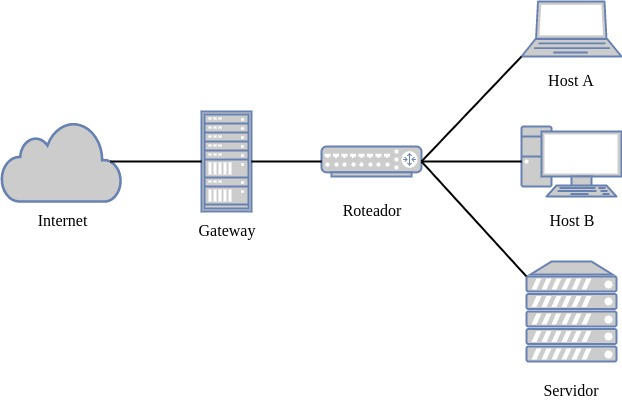
\includegraphics[width=1\textwidth]{./gateway.jpg}
	\caption{Exemplo de localização de um gateway em uma rede simples.}
	\label{fig:gateway}
\end{figure}

A proposta deste trabalho é a criação de um sistema de detecção de anomalias em redes de computadores. Para tal, será utilizada uma técnica heurística para a caracterização do tráfego da rede e uma plataforma ou método de aprendizado supervisionado de máquina será treinado para realizar a detecção automática de anomalias na rede.

	A análise do tráfego será realizada sobre o gateway, local por onde passam todos os dados que serão enviados para a internet e também todos que são recebidos da mesma. Um esquema simples de uma rede que exemplifica o funcionamento de um gateway pode ser visto na Figura 1.

%---------- Referencias ----------
\bibliography{reflatex} % geracao automatica das referencias a partir do arquivo reflatex.bib



% --------- Lista de siglas --------
%\textbf{* Observa\c{c}\~oes:} a lista de siglas nao realiza a ordenacao das siglas em ordem alfabetica
% Em breve isso sera implementado, enquanto isso:
%\textbf{Sugest\~ao:} crie outro arquivo .tex para siglas e utilize o comando \sigla{sigla}{descri\c{c}\~ao}.
%Para incluir este arquivo no final do arquivo, utilize o comando \input{arquivo.tex}.
%Assim, Todas as siglas serao geradas na ultima pagina. Entao, devera excluir a ultima pagina da versao final do arquivo
% PDF do seu documento.


%-------- Citacoes ---------
% - Utilize o comando \citeonline{...} para citacoes com o seguinte formato: Autor et al. (2011).
% Este tipo de formato eh utilizado no comeco do paragrafo. P.ex.: \citeonline{autor2011}

% - Utilize o comando \cite{...} para citacoeses no meio ou final do paragrafo. P.ex.: \cite{autor2011}



%-------- Titulos com nomes cientificos (titulo, capitulos e secoes) ----------
% Regra para escrita de nomes cientificos:
% Os nomes devem ser escritos em italico, 
%a primeira letra do primeiro nome deve ser em maiusculo e o restante em minusculo (inclusive a primeira letra do segundo nome).
% VEJA os exemplos abaixo.
% 
% 1) voce nao quer que a secao fique com uppercase (caixa alta) automaticamente:
%\section[nouppercase]{\MakeUppercase{Estudo dos efeitos da radiacao ultravioleta C e TFD em celulas de} {\textit{Saccharomyces boulardii}}
%
% 2) por padrao os cases (maiusculas/minuscula) sao ajustados automaticamente, voce nao precisa usar makeuppercase e afins.
% \section{Introducao} % a introducao sera posta no texto como INTRODUCAO, automaticamente, como a norma indica.


\end{document}